\subsection{Алгоритм Єна}
\label{subsec:yens-subsection}

Алгоритм Єна - це потужний та ефективний алгоритм, який використовується для знаходження декількох найкоротших шляхів або маршрутів між заданою парою вершин графа. Він є розширенням алгоритму Дейкстри і має перевагу в тому, що обчислює не лише єдиний найкоротший шлях, а й задану кількість альтернативних найкоротших шляхів. Це робить його особливо корисним у сценаріях, де потрібно знайти кілька оптимальних маршрутів, наприклад, у програмах планування маршрутів.

Однією з ключових переваг алгоритму Єна є його здатність ефективно генерувати k найкоротших шляхів без необхідності щоразу перераховувати весь граф. Це досягається завдяки використанню концепції обрізання графа та відхилення шляху, що дозволяє йому досліджувати різні шляхи без зайвих обчислень. Це робить алгоритм Єна добре придатним для великих графів з великою кількістю вершин і ребер.

Крім того, алгоритм Єна включає в себе концепцію відгалужень та покращень шляху, які дозволяють генерувати різноманітні альтернативні маршрути. Ітеративно видаляючи відгалуження з графа та покращуючи шляхи, що залишилися, алгоритм систематично досліджує різні можливості і створює набір з k найкоротших шляхів з мінімальним перекриттям.

Однак варто зазначити, що хоча алгоритм Єна є ефективним і дієвим для пошуку кількох найкоротших шляхів, він може стати обчислювально дорогим, коли кількість бажаних шляхів (k) зростає. Крім того, у графах з від'ємними вагами ребер або циклами алгоритм Єна може не давати коректних результатів без модифікацій.

Загалом, алгоритм Єна є цінним інструментом для планування та оптимізації маршрутів, оскільки дозволяє генерувати декілька найкоротших шляхів і дає можливість користувачам розглядати альтернативні маршрути на основі їхніх уподобань або обмежень. Здатність забезпечувати баланс між обчислювальною ефективністю та різноманітністю шляхів робить його популярним у різних сферах, де пошук оптимальних маршрутів має вирішальне значення.\\

\begin{figure}[!htp]
    \centering
    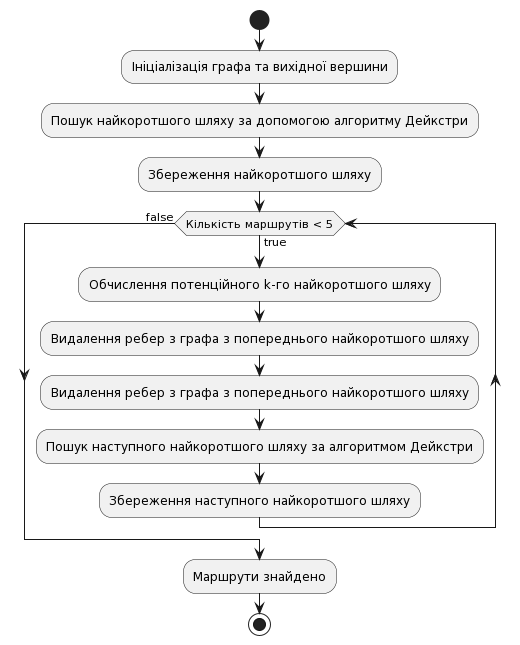
\includegraphics[scale=0.6]{content/chapters/2-implementation-methods/assets/img/yens_algorithm.png}
    \caption{Блок-схема алгоритму Єна}
    \label{fig:bfs}
\end{figure}


Переваги:
\begin{itemize}
    \item Алгоритм Єна дозволяє обчислювати кілька найкоротших шляхів між парою вузлів, надаючи користувачам альтернативні варіанти маршрутів на основі їхніх уподобань або обмежень.
    \item Алгоритм генерує різноманітні шляхи, систематично досліджуючи різні можливості за допомогою відгалужень та вдосконалень, гарантуючи, що альтернативні маршрути мінімально перетинаються.
    \item Алгоритм Єна ефективно обчислює k найкоротших шляхів, використовуючи методи обрізання графів і відхилення шляхів, що робить його придатним для великих графів з великою кількістю вершин і ребер.
    \item Алгоритм можна адаптувати для роботи з різними типами графів, включаючи орієнтовані та неорієнтовані графи, а також графи зі зваженими та незваженими ребрами.
\end{itemize}

Недоліки:
\begin{itemize}
    \item Зі збільшенням бажаної кількості шляхів (k) зростає і обчислювальна складність алгоритму Єна. Для великих значень k алгоритм може стати обчислювально дорогим і трудомістким.
    \item Алгоритм Єна може не давати коректних результатів при роботі з графами, які містять від'ємні ваги ребер або цикли. Для обробки таких сценаріїв можуть знадобитися додаткові модифікації або адаптації.
    \item У деяких випадках алгоритм може вимагати модифікації початкової структури графа для полегшення генерації альтернативних шляхів. Це може додати складності та потенційно вплинути на продуктивність алгоритму.
    \item Алгоритм Єна спеціально розроблено для пошуку найкоротших шляхів у графі. Якщо вам потрібні інші типи пошуку шляхів або оптимізаційні цілі, альтернативні алгоритми можуть бути більш придатними.
\end{itemize}
